\subsection{Tuning of ESKF for real data} \label{a2task3}
The next step was to see how the error state Kalman filter would perform on actual real life data. The available dataset contains IMU and GNSS measurements of a unmanned aerial vehicle (UAV) remotely controlled by an operator. The flight path of the UAV as seen from the GNSS measurements is shown in figure \ref{fig:eskf-real-track}.

The tuning of the kalman filter model is again based on the STIM300 datasheet, as this is the actual IMU used on the UAV. We used the same approach as in \cref{sec:using_datasheet} using the new IMU rate of $\frac{1}{\Delta t} = 250Hz$ with \cref{eq:eskf-cont-noise} to get the continious time acceleration and angular rate noise parameters. We tuned the bias models by hand, heavily inspired by our tuning from the simulated dataset. In this case, we do not have the ground truth available, so we cannot calculate the normalised error state squared (NEES). We are also not able to tune the filter using the error state. We can however use the \textit{innovation} of the kalman filter, which in layman terms is a measure of how much the filter must update or "innovate" the estimate in the update step to correct for the new measurement. In other words we can measure how "off" the prediction is which we further can compare with how certain the filter is when predicting. We also have the GNSS receivers estimated accuracy which we scaled and used as the standard deviation for the GNSS measurements. With our tuning, we are able to achieve a normalized innovation squared (NIS) that stays $81.3\%$ inside the $95\%$ $\chi^2$ confidence interval, shown in figure \ref{fig:eskf-real-nis-basic} below. We also split the NIS into one planar and one altitude component due to the difference in accuracy for GNSS. The CI $\chi^2$ was also adjusted to accommodate for the degrees of freedom in NIS. We then used the two NISes when scaling $RGNSS$. We attempted to further tune the IMU noises, but decided it was better to use the official values provided by the manufacturer. Without ground truth and error metrics, it is difficult to further quantify the performance of the filter and therefore difficult to further improve the tuning. 

\begin{subequations}
\begin{equation}
RGNSS = (0.4)^2\begin{bmatrix}
    1^2 & 0 & 0 \\
    0 & 1^2 & 0 \\
    0 & 0 & 2^2
\end{bmatrix}
\end{equation}
\begin{equation}
q_a = (1.167 \cdot 10^{-3})^2, \\
\end{equation}
\begin{equation}
q_{ab} = (1.5 \cdot 10^{-3})^2, \\
\end{equation}
\begin{equation}
p_{ab} = 10^{-8}, \\
\end{equation}
\begin{equation}
q_\omega = deg2rad((2.5 \cdot 10^{-2})^\circ)^2, \\
\end{equation}
\begin{equation}
q_{\omega b} = (4 \cdot 10^{-6})^2, \\
\end{equation}
\begin{equation}
p_{\omega b} = 10^{-8}, \\
\end{equation}
\end{subequations}



\begin{figure}[H]
        \centering
        \begin{subfigure}[b]{0.50\textwidth}
                \includegraphics[width=\textwidth]{plots/a2-real-nis}
                \caption{ NIS logarithm - logarithm is used to better visualize the spike when the AUV is launched}
                \label{fig:eskf-real-nis-basic}
        \end{subfigure}%
        \hfill
        \begin{subfigure}[b]{0.50\textwidth}
                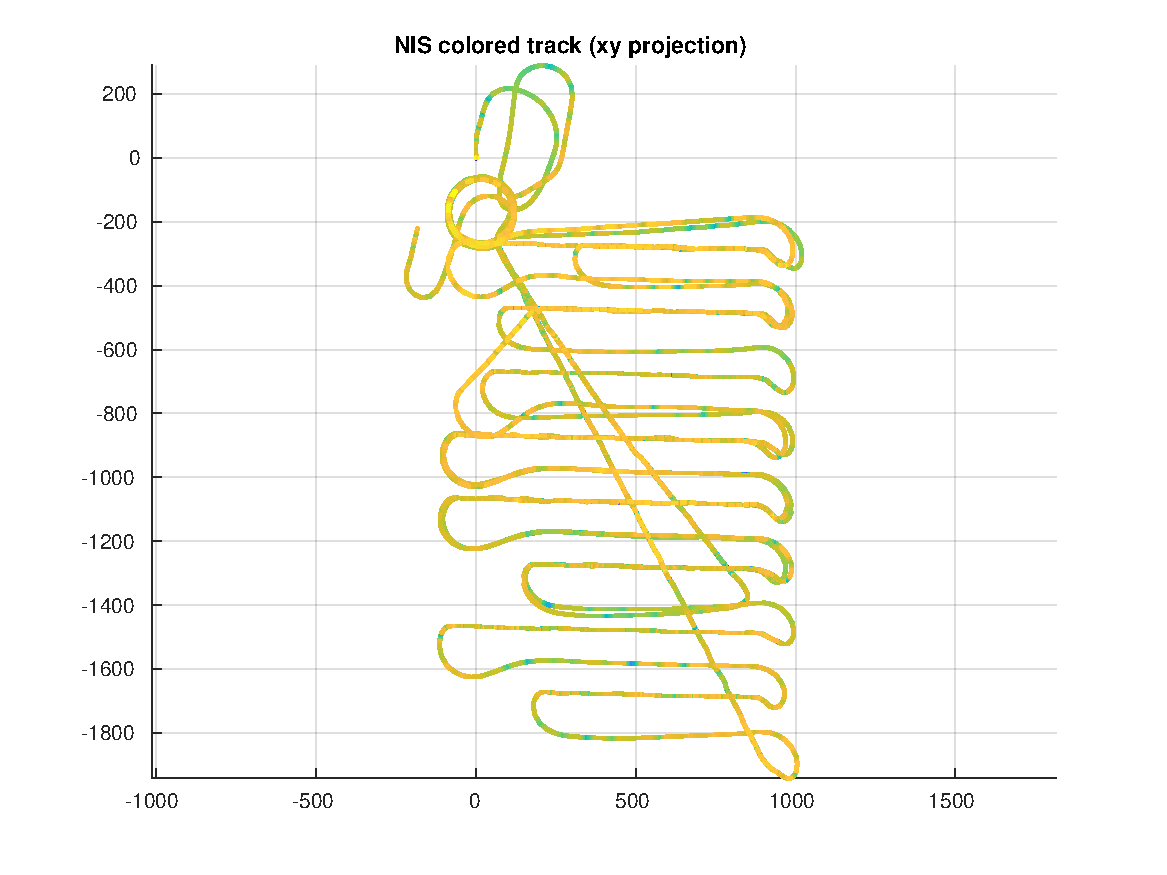
\includegraphics[width=\textwidth]{plots/a2-real-nis-colored-track}
                \caption{NIS colored track}
                \label{fig:eskf-real-nis-coloredtrack}
        \end{subfigure}
        \caption{ESKF NIS for the real dataset}
\end{figure}
\begin{figure}
        \begin{subfigure}[b]{0.49\textwidth}
                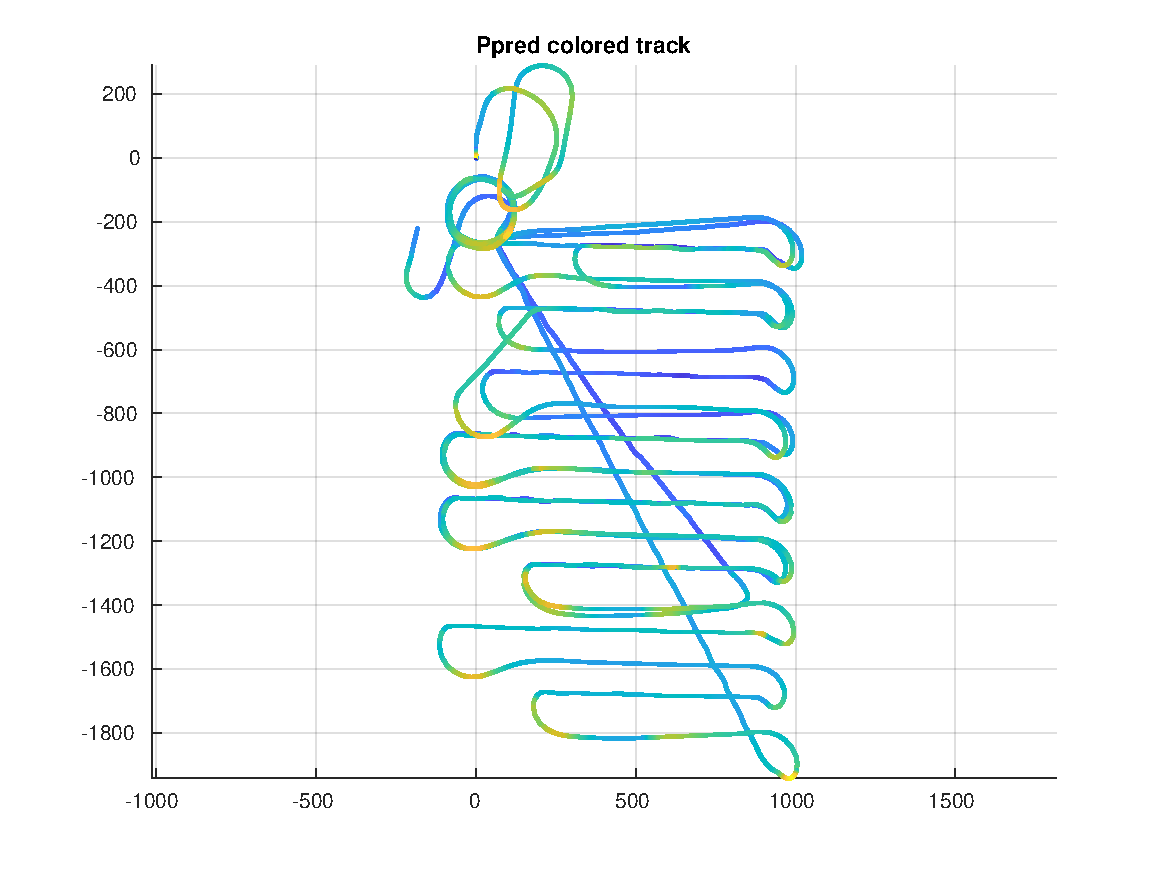
\includegraphics[width=\textwidth]{plots/a2-real-ppred-colored-track}
                \caption{$P_{pred}$ norm colored track}
                \label{fig:eskf-real-ppred-coloredtrack}
        \end{subfigure}
        \hfill
        \begin{subfigure}[b]{0.49\textwidth}
                \includegraphics[width=\textwidth]{plots/a2-real-track}
                \caption{UAV Track for the real dataset. Red=GNSS measurements, Blue=ESKF}
                \label{fig:eskf-real-track}
        \end{subfigure}
        \caption{ESKF results for the real dataset}
\end{figure}

